% !TeX root = ../../thesis.tex
\chapter{Materials and Methods}\label{ch:material_properties}

The inception of the work presented in this thesis began with the repurposing an older vacuum evaporation chamber, previously used of the fabrication of organic thin film electronics. A significant portion of initial efforts focused on calibrating the chamber for the deposition of inorganic perovskite layers, evaluating film quality and repeatability, as well as investigating the effect of fundamental deposition parameters on the performance of the photodetector devices. This chapter outlines the experimental protocol followed in this work, detailing the deposition and characterization methods of \ch{CsPbI_2Br} thin films, as well as the development of perovskite photodiodes. The latter encompasses the selection of substrates and transport layers while also emphasizing the importance of carefully interpreting electrical characterization measurements.

\section{Thermal Co-Evaporation of \ch{CsPbI_2Br} Thin Films}

\begin{figure}
  \centering
  \medskip
  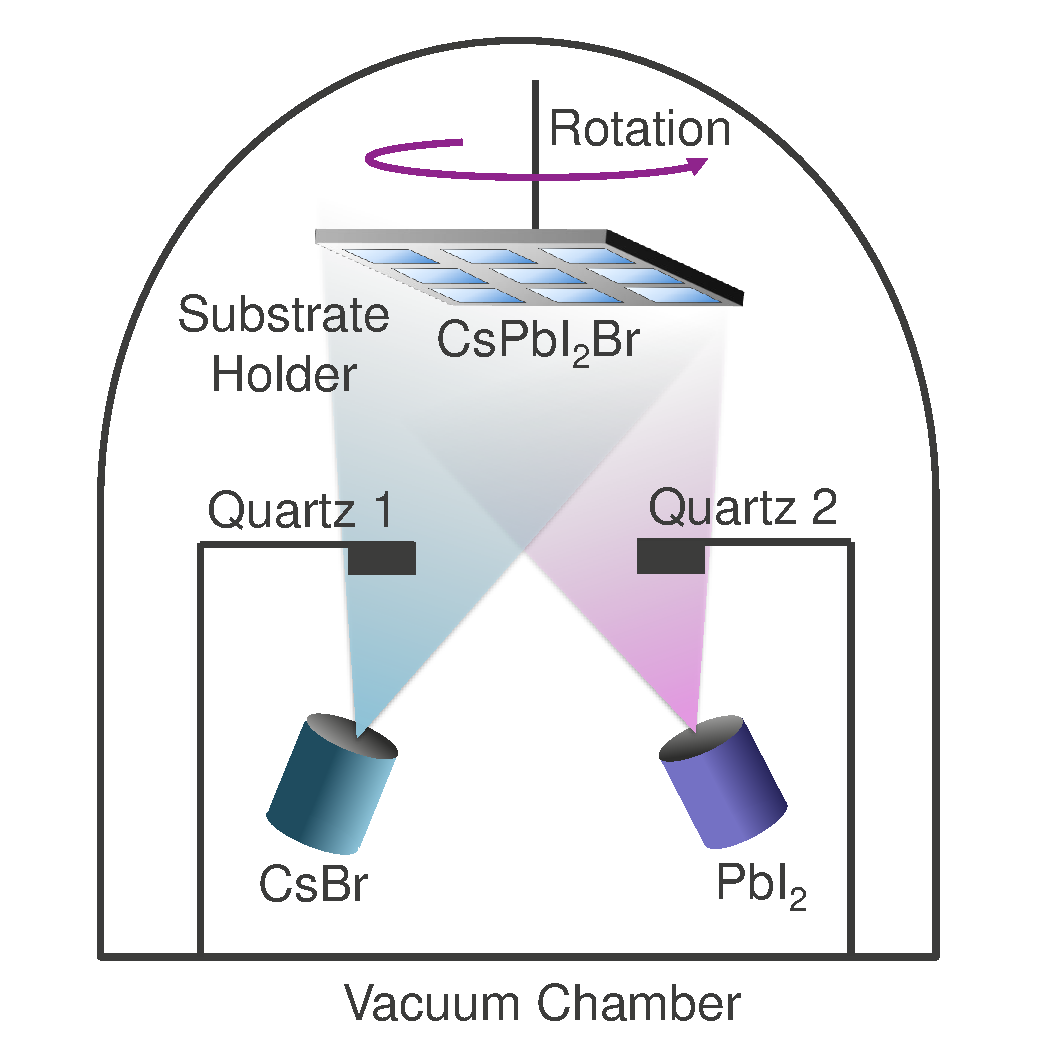
\includegraphics[width=.5\textwidth]{chapters/material_properties/images/Chamber.pdf}
  \caption[Short caption for Table of Figures]{Illustration of high-vacuum deposition chamber.}
  \label{fig:deposition_chamber}
\end{figure}

++high vacuum 


An illustration of the deposition chamber is provided in Figure~\ref{fig:deposition_chamber}. Two sources on opposite sides of the chamber are loaded with \ch{CsBr} and \ch{PbI_2} powders. Two separate quartz crystal microbalances (QCMs) are used to track the deposition rate of each source. The substrates are loaded on a substrate holder (\textbf{distance?}) that can hold up to nine $3\times 3$ $cm^2$ coupons. The QCMs have to be calibrated according to the atomic mass of the precursor they are monitoring. To achieve this, an initial estimation of their tooling factor is necessary. Subsequently, each precursor is deposited on \ch{Si/SiO_2} substrate, placed in the center of the substrate holder, and the actual thickness is measured using spectroscopic ellipsometry or profilometry. The tooling factor is then adjusted using the equation: 

\begin{equation}
    TF_{\text{actual}} = TF_{\text{approx}} \times \frac{\text{thickness(actual)}}{\text{thickness(QCM)}}
\end{equation}

To account for system variability, we deposit each precursor multiple times at different rates and target thicknesses. The final tooling factor of each source is calculated based on the average of all depositions.


Moving on to the co-evaporation of perovskite thin films, the ratio between the two sources' evaporation rates should be tuned to achieve the desired stoichiometry. For a stoichiometric film, the thickness ratio (TR) between two precursors, A and B, should be equal to: 

\begin{equation}
    TR = \frac{MolarMass(A)/Density(A)}{MolarMass(B)/Density(B)}.
\end{equation}

During the co-evaporation, a global shutter is protecting the samples while the sources are still heating up. Once both rates have reached their target value and are stabilized, the shutter is removed, initiating the deposition. The substrate holder is kept at room temperature and rotates at approximately 2.2 rounds per minute to ensure a uniform deposition. During the deposition, the temperature of each sources is continuously and automatically adjusted to maintain a constant evaporation rate. The deposition is automatically terminated once the target cumulative thickness is reached. For the development of the baseline evaporated films, a cumulative deposition rate of 0.8{\AA}/s and a \ch{CsBr:PbI_2} ratio of 1.05:1.00 was aimed for. Films were deposited with a slight excess of \ch{CsBr} since it was shown that it can improve the ambient stability of the black phase without compromising their optoelectronic properties \cite{Ma2017TheCells}. Following the deposition of the perovskite thin films, they where consistently stored in nitrogen environment to prevent their conversion to the photo-inactive yellow phase.


\section{Experimental Methodology}

Following the calibration of the tooling factor for each source, the following experimental methodology was implemented. Initially the co-evaporated \ch{CsPbI_2Br} films are deposited on glass or \ch{Si/SiO_2} substrates. This step aims to the characterization of the fundamental structural, compositional, crystallographic, and optical properties of the deposited films. Structural properties are mainly investigated using atomic force microscopy (AFM) and scanning electron microscopy (SEM), transmission electron microscopy (TEM), and spectroscopic ellipsometry (SE). Compositional properties are investigated using X-Ray and Ultraviolet photoelectron spectroscopy (XPS/UPS), energy dispersive X-Ray spectroscopy (EDS), as well as inductively coupled plasma mass spectrometry (ICP-MS). Crystallographic properties are investigated using synchrotron-based grazing incident wide angle X-ray scattering (GIWAXS). Optical properties are investigated using photoluminescence (PL), ultraviolet-visible spectroscopy (UV-Vis), and SE. Finally, the ambient stability of the deposited films is investigated through their exposure to the controlled environment of the lab (temperature, humidity). 


After ensuring the high quality of the bare perovskite films, they are flowingly incorporated in the bottom-illuminated photodiode stack, using glass substrates, pre-patterned with ITO. The ITO serves as the common contact, while the device area is defined by the aluminum (Al) electrodes deposited on top of the perovskite. This step is instrumental for the screening of various parameters and their influence on device performance, including the perovskite annealing conditions or choice of transport layers. Characterization measurements used for this step mainly rely on acquisition of J-V characteristics, EQE spectral response, as well as capacitance and transient photocurrent measurements.

Once the most prominent perovskite processing conditions and transport layers have been identified, it is possible to proceed to the development of the top-illuminated stack, replacing the glass substrate with a silicon one. This serves as an intermediate step before integrating the PePD top of the Si ROIC for imager fabrication. The silicon substrates are patterned with titanium nitride bottom contacts (TiN) and they are designed internally and fabricated in imec's CMOS foundry. The bottom TiN contacts define the device area, while to common contact is defined by the ITO that is deposited on top of the perovskite.  

while 


they are transferred to the top-illuminated stack, relying on the use of silicon substrates, patterned with titanium nitride (TiN) bottom contacts. In this case, the common contact (ITO) is deposited on top of the perovskite layer. These substrates, designed internally and fabricated in imec's CMOS foundry. Characterizing the performance of the photodiode stack deposited on top of silicon substrates is critical for evaluating its performance on the C

the use of different contacts, as well as the opposite illumination creates diffrence in the peroformance which require the repetition of the above mentioned characterization measuremetns. 


and allow for characterization on discrete diode level, mimicing the strucutre of the photodiode on top of the ROIC. Besides the measurements that were described above, the use of Silicon substrates allows for the additional characterization of thermal stability, as well as ambinets atmosphere stability of the whole stack. 


TOP illuminiated photodiodes for CMOS integration. 

\textit{Once the perofromance as well as the stability of the photodiode stack was assured, it was possible to tranfer the photodiode on top of the ROIC, pixels are in the 0.56 um. 
}



\section{Development of Perovskite Photodiodes}

\subsection{Substrates and Electrodes}

\subsection{Transport Layers}

A review of available transport layers and the ones we use + energetic landscape.

on top of the perovskite is more critical, since sputtering is usually too aggressive for the lattice - thermal evaporation, or deposition via ALD have been previously explored 

fewer options are avaialble for inorgnic HTLs - NiOx - that thy we rely solely on the use of 


\textbf{Good discussion and references for Metal Oxides as transport layers happens here \cite{Yang2023InvertedPassivation}}.






\begin{figure}[htbp]
    \centering
    % First plot
    \begin{subfigure}[t]{0.49\textwidth} % Adjust width as needed
        \centering
        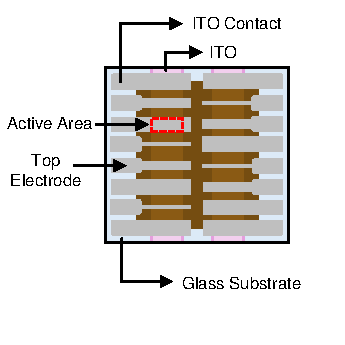
\includegraphics[width=\textwidth]{chapters/material_properties/images/Glass_Substrate.pdf} % Replace with your image
        \caption{}
        \label{fig:ch2:glass_substrate}
    \end{subfigure}
    \hfill % Space between the two plots
    % Second plot
    \begin{subfigure}[t]{0.49\textwidth} % Adjust width as needed
        \centering
        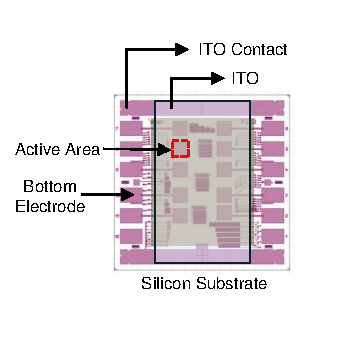
\includegraphics[width=\textwidth]{chapters/material_properties/images/PIX_Substrate.pdf} % Replace with your image
        \caption{}
        \label{fig:ch2:pix_substrate}
    \end{subfigure}

    % Caption for the whole figure
    \caption{Substrate layouts: (a) glass substrate, and (b) silicon substrate.}
    \label{fig:ch2:types_of_substrates}
\end{figure}


This section provides an overview of the parameters that can be varied during the development of perovskite-based photodetectors and their impact on device performance. As shown in Fig.\ref{fig:ch2:types_of_substrates}, two types of substrates were used in this study: glass substrates pre-patterned with an ITO contact (Fig.\ref{fig:ch2:glass_substrate}) and silicon substrates, designed internally and fabricated in imec's CMOS foundry, featuring a TiN bottom contact (Fig.~\ref{fig:ch2:pix_substrate}).

Independetnly of the used substrate, the fabrication process is similar. For both of the 15 nm of NiOx are deposited via DC sputtering. The NiO-covered film is annealed for 5 minutes at 300 C in open air to promote the oxidataiton of the substrate. Then the perovskite is deposited, in most cases followed by a post deposition flash annealing step at 300 C for 5 seconds.- add stack diagram, taken from the paper on the ETL optimization.

The fabrication process is similar for both substrate types, beginning with the deposition of the HTL (DC sputtered \ch{NiO_x}), followed by the deposition of the perovskite layer, the post-deposition annealing step, and finally, the deposition of the ETL. For glass substrates, the stack is completed by depositing Al contacts via thermal evaporation, using a shadow mask that defines 12 different devices. The device area is determined by the overlap between the ITO and Al electrodes, resulting in three different areas: 0.125 $cm^2$, 0.075 $cm^2$, and 0.025 $cm^2$. The use of variable-sized contacts allows for an analysis of the impact of device area on performance metrics.

For silicon substrates, the stack is completed with the deposition of an ITO sheet via linear magreton sputtering. In this case, the device area is defined by the bottom TiN contact, which is fixed at 0.0625 $cm^2$. The illumination setup differs between the two substrates: glass substrates are illuminated from the bottom (through the glass side - Fig.~\ref{fig:ch2:glass_stack}), while silicon substrates are illuminated from the top (through the ITO side - Fig.~\ref{fig:ch2:pix_stack}). 

The silicon substrates mimic the device structure used in the fabrication of imagers.2 However, due to their greater availability and accessibility, glass substrates are preferred for rapid prototyping and the screening of various deposition parameters and layers. Stacks that demonstrate promising performance are subsequently transferred and evaluated on silicon substrates. Despite the opposite orientation of the common contact, the results for both substrates are presented such that a negative bias consistently represents the reverse bias regime of the sample.


\begin{figure}[htbp]
    \centering
    % First plot
    \begin{subfigure}[t]{0.4\textwidth} % Adjust width as needed
        \centering
        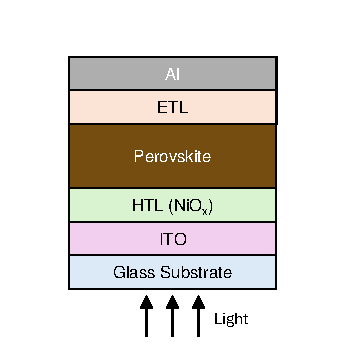
\includegraphics[width=\textwidth]{chapters/material_properties/images/Glass_Stack.pdf} % Replace with your image
        \caption{}
        \label{fig:ch2:glass_stack}
    \end{subfigure}
    \hfill % Space between the two plots
    % Second plot
    \begin{subfigure}[t]{0.4\textwidth} % Adjust width as needed
        \centering
        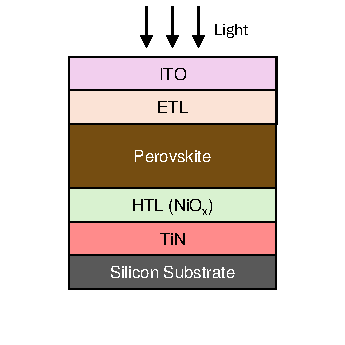
\includegraphics[width=\textwidth]{chapters/material_properties/images/PIX_Stack.pdf} % Replace with your image
        \caption{}
        \label{fig:ch2:pix_stack}
    \end{subfigure}

    % Caption for the whole figure
    \caption{Stack and illumination direction for (a) glass substrate, and (b) silicon substrate.}
    \label{fig:ch2:types_of_stacks}
\end{figure}

\section{Impact of Characterization Method and Statistical Remarks}

The characterization of the electrical performance of perovskite-based devices is not straight forward due to the presence of mobile ions in the lattice, which migrate under an applied and electric field, accumulate at the contacts and potentially participate in electrochemical reactions. In mixed-halide perovskites, phase segregation is another common occurrence. These are just some of the effects that occur under illumination or external bias, making it challenging to disentangle phenomena attributed to charge carriers, mobile ions, or newly formed species within the perovskite layer. A characteristic consequence of this complexity is hysteresis in J-V measurements, which has been shown to depend not only on the scan direction and speed, but also on the composition of the perovskite, the choice of transport layers, etc. 

\begin{figure}[htbp]
    \centering

    % First row
    \begin{subfigure}[b]{0.4\textwidth}
        \centering
        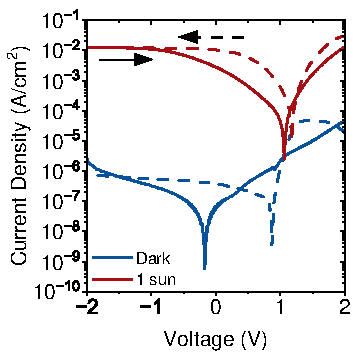
\includegraphics[width=\textwidth]{chapters/material_properties/images/Forward-Reverse-Plot.pdf}
        \caption{}
        \label{fig:ch2:scan_direction}
    \end{subfigure}
    \hfill
    \begin{subfigure}[b]{0.4\textwidth}
        \centering
        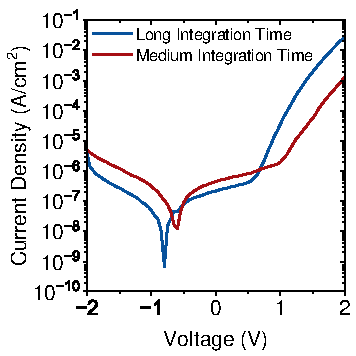
\includegraphics[width=\textwidth]{chapters/material_properties/images/Integration-Speed.pdf}
        \caption{}
        \label{fig:ch2:scan_speed}
    \end{subfigure}

    % Second row
    \begin{subfigure}[b]{0.35\textwidth}
        \centering        
        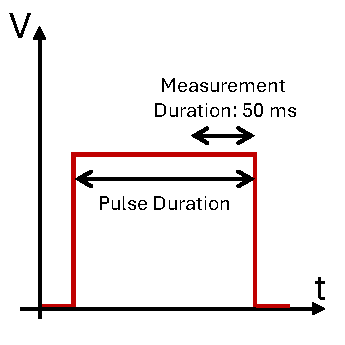
\includegraphics[width=\textwidth]{chapters/material_properties/images/PAIOS_Pulsed_Measurement.pdf}
        \caption{}
        \label{fig:ch2:pulsed_meas_PAIOS}
    \end{subfigure}
    \hfill
    \begin{subfigure}[b]{0.4\textwidth}
        \centering
        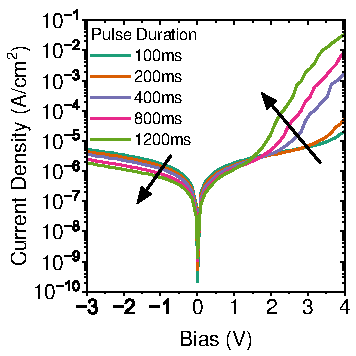
\includegraphics[width=\textwidth]{chapters/material_properties/images/Pulsed-PAIOS-plot.pdf}
        \caption{}
        \label{fig:ch2:pulsed_paios}
    \end{subfigure}


    % Third row - centered figure
    \begin{subfigure}[b]{0.4\textwidth}
        \centering
        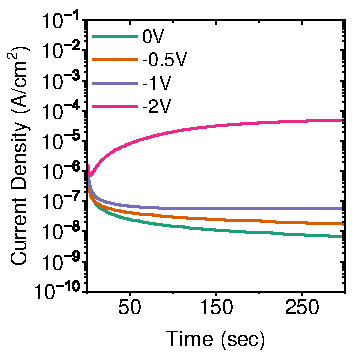
\includegraphics[width=\textwidth]{chapters/material_properties/images/Steady-State-plot.pdf}
        \caption{}
        \label{fig:ch2:steady_state}
    \end{subfigure}

    \caption{Impact of characterization methodology on device performance}
    \label{fig:ch2:types_of_measurement}
\end{figure}

Most commonly, the characterization of photodetectors relies on sequential J-V scans, which can be performed in dark and under illumination. Fig.~\ref{fig:ch2:scan_direction} shows the impact of the scan direction for one of the fabricated devices, while Fig.~\ref{fig:ch2:scan_speed} demonstrates the impact of the integration time. A significant hysteresis is observed, with the value of dark current, one of the most critical figures of merit of photodetectors, being highly dependent on the characterization settings. It is possible to eliminate hysteresis in the JV data by performing a pulsed IV measurement, the principle of which is demonstrated in Fig.~\ref{fig:ch2:pulsed_paios}. Specifically, each voltage step is applied as a pulse of specific length (pulse duration). The current value for each voltage step is the extracted as the average transient current during the specified measurement duration. This approach allows the ions to re-distribute for each voltage step, eliminating the hysteresis from the JV data (minimum $J_d$ is at 0 V, as shown in Fig.~\ref{fig:ch2:pulsed_meas_PAIOS}). However, even for this type of measurement, it is clear that the duration of each voltage pulse has a major impact on the measured J-V performance, with longer pulses leading to lower values of $J_d$ and larger values of forward current (rectification). (Why?) A last option for the characterization of the perovskite-based photodiodes is steady-state measurements, where a constant bias is applied and maintained for a prolonged period, until the value of monitored current starts saturating. This is demonstrated in Fig.~\ref{fig:ch2:steady_state}. A large drop in the value of $J_d$ is observed within the first seconds of the measurement, which was previously to depend on capacitive effects, rather than the presence of mobile ions \cite{Ollearo2021UltralowGeneration}. At -2 V, an almost 3-order increase in $j_d$ is observed, which has been associated with the breaking down of the device. This mechanism is concealed when performing J-V scans of relatively small duration and will be further investigate in Chapter~\ref{ch:transport_layer}. Considering the variability of results depending on the characterization approach, we mainly utilize sequential J-V scans, performed in the forward direction for comparing various stacks, stating that despite the impact of the measurement on the results, it still allows the fair identification of trends among different conditions. 


\begin{figure}[htbp]
    \centering
    % First plot
    \begin{subfigure}[t]{0.4\textwidth} % Adjust width as needed
        \centering
        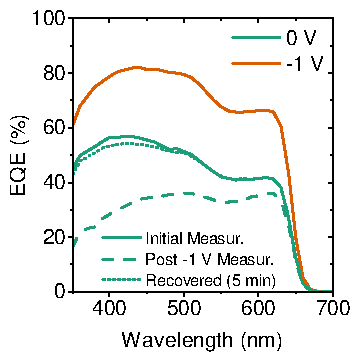
\includegraphics[width=\textwidth]{chapters/material_properties/images/EQE-1V.pdf} % Replace with your image
        \caption{}
        \label{fig:ch2:eqe-1V}
    \end{subfigure}
    \hfill % Space between the two plots
    % Second plot
    \begin{subfigure}[t]{0.4\textwidth} % Adjust width as needed
        \centering
        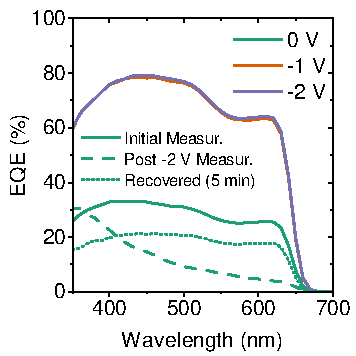
\includegraphics[width=\textwidth]{chapters/material_properties/images/EQE-2V.pdf} % Replace with your image
        \caption{}
        \label{fig:ch2:eqe-2V}
    \end{subfigure}

    
    \begin{subfigure}[t]{0.9\textwidth}
        \centering
        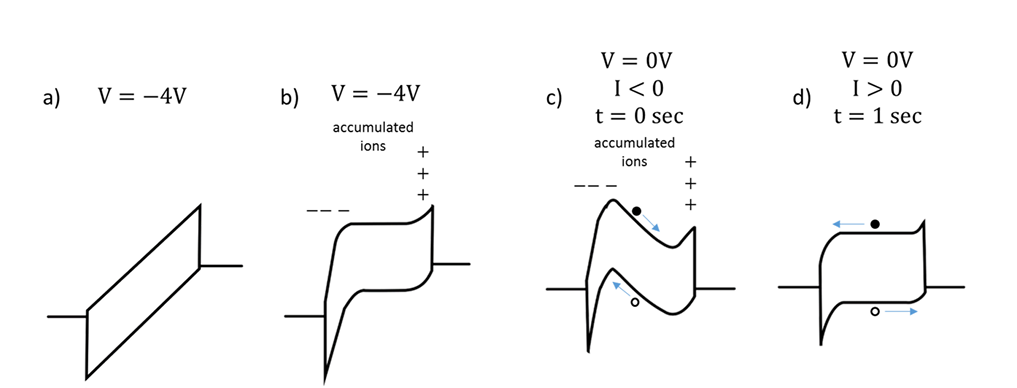
\includegraphics[width=\textwidth]{chapters/material_properties/images/ions.png} % Replace with your image file
        \caption{}
        \label{}
    \end{subfigure}

    % Caption for the whole figure
    \caption{Impact of measurement order on the EQE measurements.}
    \label{fig:ch2:eqe}
\end{figure}

The impact of the characterization approach on the acquired results extends to EQE measurements, as well. Fig.~\ref{fig:ch2:eqe-1V} and \ref{fig:ch2:eqe-2V} demonstrate the EQE results for two different devices that were fabricated on the same substrate. The EQE of the first device was measured sequentially at 0 V and -1 V, while the second device underwent measurements at 0 V, -1 V, and -2 V. Following these measurements, each device was subjected to two additional EQE measurements at 0 V: one immediately after the highest applied reverse bias (-1 V and -2 V, respectively) and another after a five-minute resting period in the dark. For both devices, the EQE at 0 V immediately after reverse biasing was significantly lower than the initial EQE measurement at 0 V. However, for the device biased up to -1 V, a five-minute resting period was sufficient to fully restore the initial EQE value. In contrast, for the device biased up to -2 V, the EQE at 0 V remained approximately 40\% lower than its initial value even after five minutes of recovery. This phenomenon could potentially be attributed to the accumulation of ions at the contacts and their potential contribution to electrochemical reactions, as demonstrated in Fig. xx. This experiment highlights the sensitivity of the acquired results to the prior biasing conditions. (Fing how much time it would take for the ions to re-distribute, and mention that is probably an electrochemical reaction that is taking place). From now on, the presented EQE results are performed on a new device, without prior bias, performed from the lowest to the highest reverse bias conditions. 

\begin{figure}[htbp]
    \centering
    % First row
    \begin{subfigure}[t]{0.4\textwidth}
        \centering
        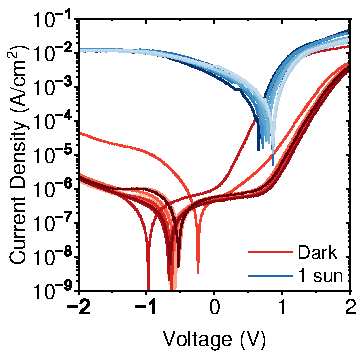
\includegraphics[width=\textwidth]{chapters/material_properties/images/High_yield_discrete.pdf} 
        \caption{}
        \label{fig:ch2:high_yield_discrete}
    \end{subfigure}
    \hfill
    \begin{subfigure}[t]{0.4\textwidth}
        \centering
        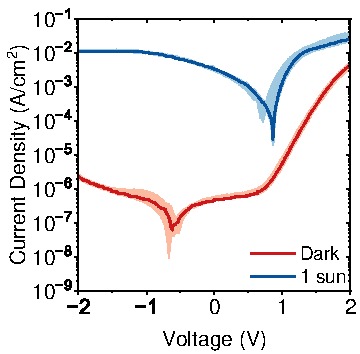
\includegraphics[width=\textwidth]{chapters/material_properties/images/High_yield_median.pdf} % Replace with your image file
        \caption{}
        \label{fig:ch2:high_yield_median}
    \end{subfigure}

    \vspace{1em} % Space between rows

    % Second row
    \begin{subfigure}[t]{0.4\textwidth}
        \centering
        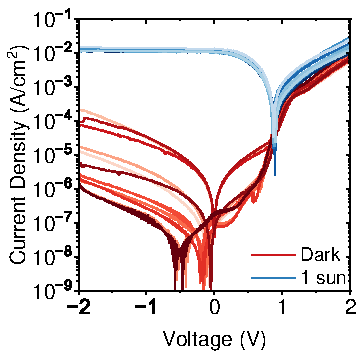
\includegraphics[width=\textwidth]{chapters/material_properties/images/low_yield_discrete.pdf} % Replace with your image file
        \caption{}
        \label{fig:ch2:low_yield_discrete}
    \end{subfigure}
    \hfill
    \begin{subfigure}[t]{0.4\textwidth}
        \centering
        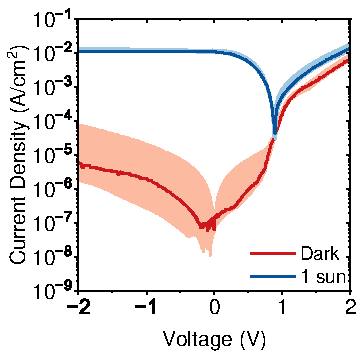
\includegraphics[width=\textwidth]{chapters/material_properties/images/low_yield_median.pdf} % Replace with your image file
        \caption{}
        \label{fig:ch2:low_yield_median}
    \end{subfigure}
    \caption{Discrete and statistical representation of J-V curves for samples with high and low variability.}
\end{figure}


Another important point is the related to the fair representation of the J-V data among the 12 devices on the same sample. Typically, there are a few outliers in each sample, the number of which defines the variability of a sample. This is more clearly illustrated in Fig.~\ref{fig:ch2:high_yield_discrete} and Fig.~\ref{fig:ch2:low_yield_discrete}, which represent two samples with small and large variability in device performance, respectively. In order to represent the median response of the sample, while also providing some insights into its variability we opt for presenting its performance in a statistical way, as shown in Fig.~\ref{fig:ch2:high_yield_median} and Fig.~\ref{fig:ch2:low_yield_median}, where the solid line represents the median response, while the shaded area represents the interquartile range. This way, the presence of 1 or 2 outliers in the device performance does not define the variability of the sample, which is reasonable considering the large area of the device and the likelihood of localized defects arising from process variations. 

Lastly, it is important to highlight the repeatability of device performance over different time periods. The fabrication tools used in this study were shared across multiple activities within the group, with occasional periods of downtime or non-standard behavior. Given the numerous variable parameters in a lab environment, pinpointing the exact causes of performance fluctuations is challenging. Inevitably, these variations also affected the performance of baseline devices. Consequently, the same device stack, when fabricated at different stages of the PhD work, may have exhibited varying degrees of performance fluctuation. This is noted to emphasize that, in this study, only samples fabricated within close temporal proximity are compared to identify trends and draw meaningful conclusions.




%%%%%%%%%%%%%%%%%%%%%%%%%%%%%%%%%%%%%%%%%%%%%%%%%%
% Keep the following \cleardoublepage at the end of this file, 
% otherwise \includeonly includes empty pages.
\cleardoublepage

